\documentclass[a4paper,11pt,twoside,openright]{report}
\usepackage{standalone}
\usepackage[lmargin=142pt,rmargin=95pt,tmargin=127pt,bmargin=123pt]{geometry}
\usepackage{csvsimple}
\usepackage{graphicx}
\usepackage[table]{xcolor}
\usepackage[flushleft]{threeparttable}
\usepackage{makecell}
\usepackage[super]{nth}
\usepackage[most]{tcolorbox}
\usepackage{listings}
\usepackage{enumitem}
\usepackage{fdsymbol}
\usepackage{awesomebox}
\usepackage{titlesec}
\usepackage{hyperref}
%\usepackage{inconsolata}
\usepackage{tikz}
\lstset{aboveskip=18pt,belowskip=18pt}
\tcbset{colframe=blue!50!black,colback=blue!20}
\hypersetup{
    colorlinks=true,
    linkcolor=blue,
    filecolor=magenta,      
    urlcolor=cyan,
    pdftitle={PAL-1 Digital Complex Sound Generator},
    pdfpagemode=UseThumbs,
    pdfauthor={Plastic Objects Limited}
    }
\titleformat{\chapter}{\normalfont\huge}{\thechapter.}{20pt}{\huge\it}
\makeatletter
\newcommand{\code}{\texttt}
\newcommand\frontmatter{
  \cleardoublepage
  \pagenumbering{roman}}
\newcommand\mainmatter{
  \cleardoublepage
  \pagenumbering{arabic}}
\newcommand\encircle[1]{%
  \tikz[baseline=(X.base)] 
    \node (X) [draw, shape=circle, inner sep=0] {\strut #1};}
\title{PAL-1 Digital Complex Sound Generator}
\author{Plastic Objects Limited}
\date{}
\begin{document}
\frontmatter
\begin{titlepage}
\begin{figure}[t]
\centering
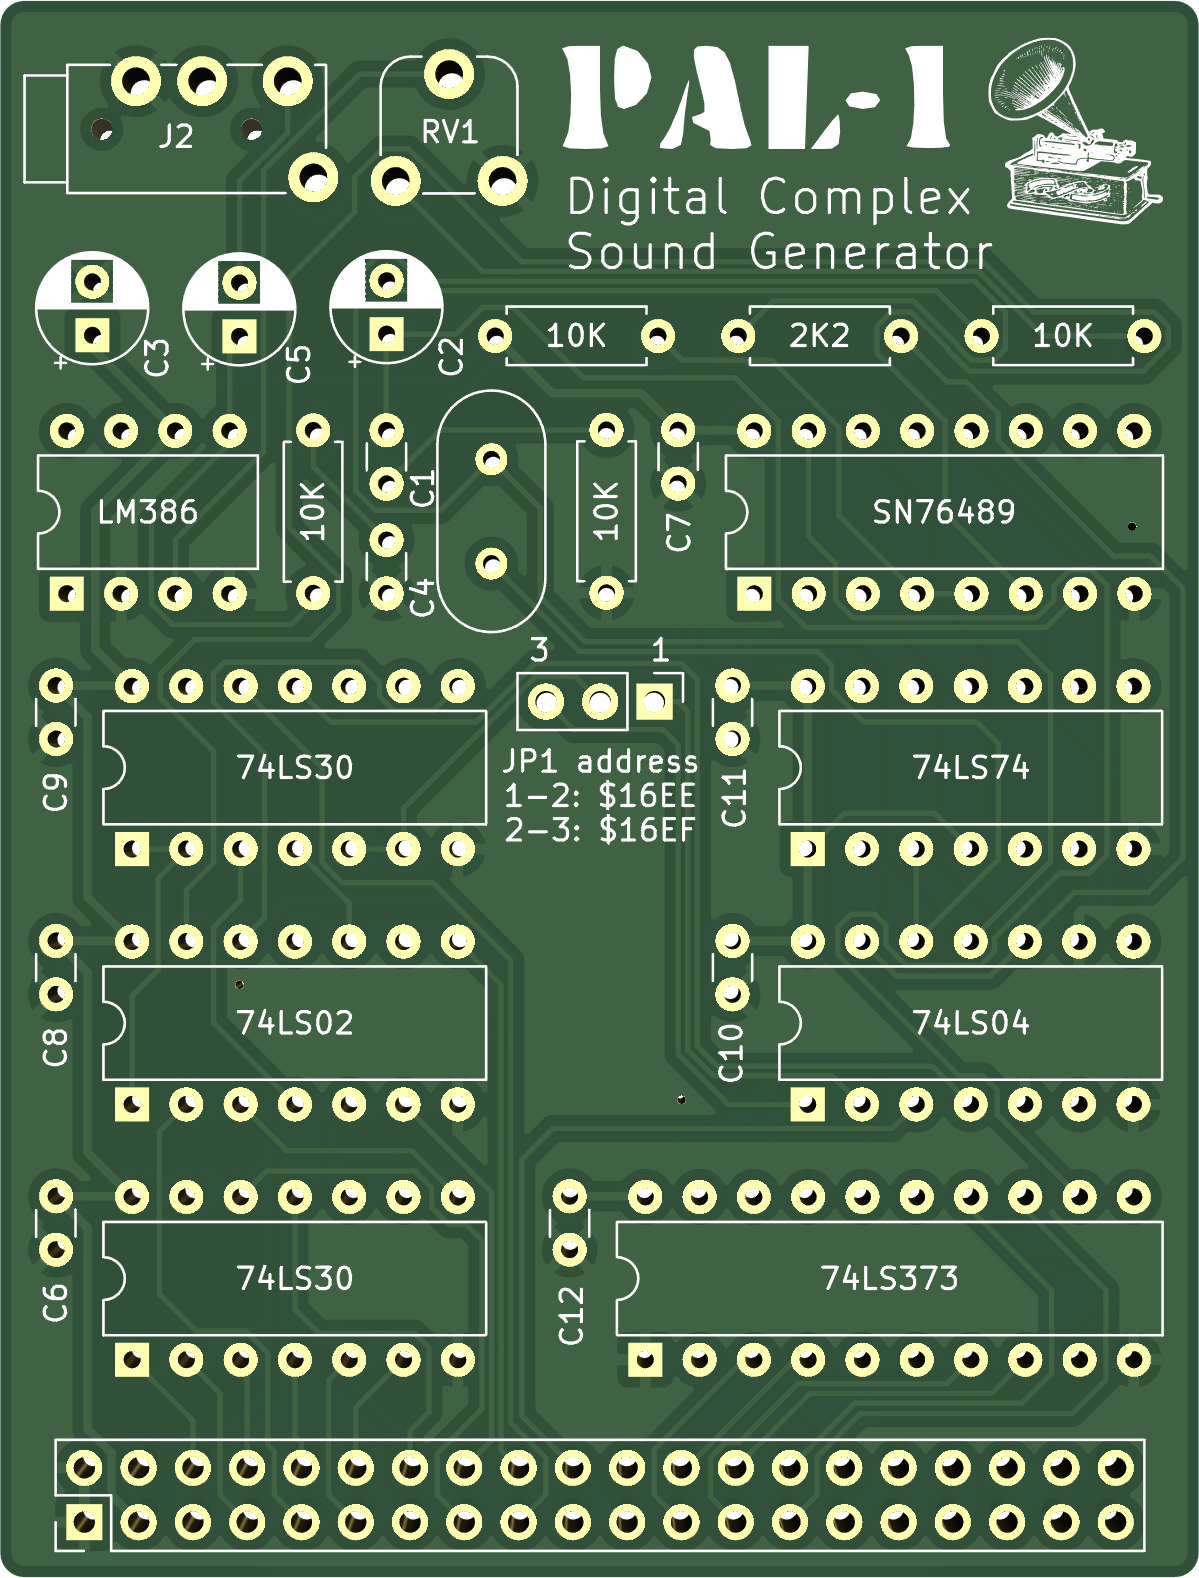
\includegraphics[scale=0.2]{figures/sound.png}
\end{figure}
\maketitle			
\end{titlepage}
\clearpage
\noindent Published by \textbf{Plastic Objects Limited} \\
Woodbridge, UK

\bigskip
\noindent August 2022
\vfill
{\noindent\Large\textbf{Disclaimer}}
\vskip 6pt
Every effort has been made to ensure the accuracy of the information contained in this document. The information presented 
within is accurate at the time of publication. Whilst every effort is made to provide accurate information, no warranty or 
fitness is provided or implied, and the authors and publishers shall have neither liability nor responsibility to any person 
or entity with respect to any loss or damages arising from its use.

All trademarks, logos and brand names are the property of their respective owners. All company, product and service names
mentioned in this document are for identification purposes only. Use of these names, trademarks and brands does not imply 
endorsement.

\thanks{PAL-1 and the PAL-1 logo used with kind permission of Liu Ganning.}
\clearpage
\tableofcontents
\cleardoublepage
\chapter*{Introduction}
\addcontentsline{toc}{chapter}{Introduction}  
The PAL-1 Digital Complex Sound Generator is an expansion module for the PAL-1
system\footnote{Liu Ganning, ‘PAL-1 Microcomputer User Manual’, 2020,  
\url{http://pal.aibs.ws/assets/PAL\textunderscore en.pdf} {[accessed 21 July 2022]}.}, based on the Texas 
Instruments SN76489 Digital Complex Sound Generator (DCSG)\footnote{The EngineeringStaff of TEXAS 
INSTRUMENTS Semiconductor Group, ‘SN76489AN’ (TEXAS INSTRUMENTS, N.D.)} and was inspired by a Ciarcia's
Circuit Cellar project\footnote{Ciarcia, Steve, ‘Add Programmable Sound Effects to Your Computer’, 
Byte, 7.7 (1982), 60–72}. 

The SN76489 DCSG was used in a range of arcade games, game consoles, and home and business computers 
from the late 1970s and throughout the 1980s. Notable systems using discrete SN76489 ICs include the 
ColecoVision games console and BBC Micro home computer. Others, such as the SEGA Mega Drive, include 
the SN76489 in their Video Display Processor (VDP) or used SN76489 clones, for example the Tandy 1000 
and IBM PCjr.

The SN76489 provides three programmable tone generators and a noise source. The signals generated by 
the tone generators and noise source are mixed in the IC and passed to an output buffer. Since the 
maximum drive of the SN76489 output pin is just 10mA, the PAL-1 Digital Complex Sound Generator 
includes a simple audio power amplifier circuit to allow a speaker to be directly connected.

\mainmatter
\chapter{Getting Started}
\section*{Board assembly}
Before assembling your PAL-1 Digital Complex Sound Generator board check the package contents against the 
Bill of Materials on page \pageref{sec:bom}, and contact your distributor as soon as possible if any 
items are missing.

No specialist tools are required for assembling the board, though care must be taken when handling ESD 
sensitive components, especially the ICs. Before inserting the ICs into their sockets, check the board 
for dry joints and solder bridges. 

\awesomebox[red]{2pt}{\faHandPaper}{red}{To prevent damage to your system, \textit{always} power off 
your PAL-1 before installing or removing the PAL-1 Digital Complex Sound Generator board. Ensure that
the pins are correctly aligned when inserting the board into the PAL-1 motherboard or when directly 
connecting it to the PAL-1 expansion port using a 40-pin IDC cable.}

\section*{Audio output}
The PAL-1 Digital Complex Sound Generator incorporates an LM386 audio power amplifier to allow an 
$8\Omega$ speaker to be directly connected. To connect a speaker or external amplifier use a cable 
with a 3.5mm mono audio jack. Sound will be heard on one channel only when stereo speakers or
a stereo amplifier are used.   

Audio volume can be controlled by adjusting the potentiometer (RV1). Refer to \textit{Attenuation}
on page \pageref{sec:attenuation} for details on setting audio volumes of individual channels.
\textbf{Note that on power-up the SN76489 registers will contain random values, meaning that random
noise may be heard until the attenuation registers are updated.}

\section*{I/O address configuration}
\label{sec:configuration}
The SN76489 DCSG has an 8-bit write only data bus, which is memory mapped on the PAL-1 system. The   
address at which it is mapped can be configured using jumper JP1, as shown in Table \ref{tab:addresses}.
Note that these addresses are \textit{not} mirorred at \$FEEE or \$FEEF.

The default address (and the address used in all examples in this manual) is \$16EE (5870 decimal). 
In situations where multiple sound generator boards are installed in the same PAL-1 system, each 
board must have a unique address. 

\begin{table}[h]
\centering
\begin{tabular}{c | c}
JP1 pins & Address \\ \hline
1-2 & \$16EE \\
2-3 & \$16EF
\end{tabular}
\caption[]{I/O address configuration}
\label{tab:addresses}
\end{table}

\chapter{Using the PAL-1 Digital Complex Sound Generator}

\section*{SN76489 internals}
The SN76489 contains 8 internal registers which control the volume and frequencies of each of 
its three tones and the volume, type and shift-rate of the noise generator. Register values are 
changed by writing to the SN76489 8-bit data bus, which on the PAL-1 is memory mapped at either
\$16EE or \$16EF. 

Each tone generator requires 10 bits of information to set the frequency and 4 bits of 
information to set the attenuation. Since the SN76489 bus is 8 bits wide, frequency updates
require double byte transfers, whilst changing attenuator values is achieved by writing 
single bytes. When writing data to the SN76489 the most significant bit (msb) of the first 
byte, the 'latch and data' byte, is always 1. For register updates that require a second byte, 
a 'data' byte, the msb is always 0.

\subsection*{Latch and data bytes}
A 'latch and data' byte is identified by its first bit, which is always 1. This is followed by
bits indicating the register (r) to be updated, composed of the destination channel (r0 \& r1) 
and the register type (r2). The final bits (d0 thru d3) are the actual data to be written 
to the relevant register. When writing to the noise source register, which requires only 3 bits 
of data, the highest bit (d0) is discarded.

\begin{figure}[h!]
\centering	
\tcbox{
\begin{tabular}{@{\extracolsep{4pt}}cccccccc@{}}
	1 & r0 & r1 & r2 & d0 & d1 & d2 & d3 \\
	\cline{1-1}\cline{2-3}\cline{4-4}\cline{5-8}
	 1 & \multicolumn{2}{c}{channel} & type & \multicolumn{4}{c}{data}  
\end{tabular}}
\caption{Latch and data byte format}
\end{figure}

Refer to Table \ref{tab:registerbits} for details of the channel and type bits
(r0-r2).

\begin{table}[h!]
	\centering
	\begin{tabular}{@{\extracolsep{4pt}}cclcl@{}}
		r0 & r1 & channel & r2 & type \\ 
		\cline{1-3}\cline{4-5}
		0 & 0 & tone 1 & 0 & tone / noise \\
		0 & 1 & tone 2 & 1 & attenuation \\
		1 & 0 & tone 3 & & \\
		1 & 1 & noise  & &
	\end{tabular}
	\caption{Latch and data byte register (r) bits}
	\label{tab:registerbits}
\end{table}

\subsection*{Data bytes}
The first bit of a 'data' byte is 0. Since frequency data consists of 10 bits, with the first 4 bits
specified in the 'latch and data' byte, only 6 bits of frequency information are required in a 'data'
byte (as shown in Figure \ref{fig:databyte}). 

Data is written to the register most recently latched using a 'latch and data' byte. This means that 
the lower 6 bits of a frequency can be updated without re-specifying the relevant tone register, for 
example for frequency sweeps.

Note that data is not ignored when the most recent register latched was something other than a tone 
frequency register. Rather, the number of bits required for the relevant type will be written to the 
latched register. For example, audio volume can be faded in or out by consecutive data writes to an
attenuation register.

\begin{figure}[h!]
	\centering	
	\tcbox{
	\begin{tabular}{@{\extracolsep{4pt}}cccccccc@{}}
		0 & x & d0 & d1 & d2 & d3 & d4 & d5 \\
		\cline{1-1}\cline{2-2}\cline{3-8}
		 0 & x & \multicolumn{6}{c}{data}  
	\end{tabular}}
	\caption{Data byte format}
	\label{fig:databyte}
\end{figure}
	
\subsection*{Calculating frequency values}
\label{sec:calculation}
The SN76489 relies on an external clock signal to generate sounds, which On the PAL-1 Digital Complex 
Sound Generator board is 2Mhz. The external clock is divided by 16 to arrive at an internal
clock of 125Khz.

Each tone and the noise generator has a 10 bit counter and an output bit. When not 0, each counter is 
decremented at the rate of the internal clock. When a counter reaches 0, the output bit for the relevant 
tone or the noise generator is flipped from 0 to 1 (or vice versa) and the counter is reset to the value
currently in corresponding register. The result is a square wave, with a wavelength of double the 
register value. Its frequency can be calculated using the following formula

\begin{align*}
	f &= \frac{N}{32n} \\
	\text{where}~N &= \text{reference clock in Hz (i.e. 2Mhz)} \\
	n &= \text{10-bit binary counter value}
\end{align*}

For example, to set tone generator 1 to a frequency of 466.164Hz (\textit{$A\sharp_4$}), 
first find \(I\):

$$
 I = \frac{N}{32f}
 = \frac{2,000,000}{32 * 466.164}
 = 134.073
$$

Since \(I\) must be an integer value, it is rounded down to 134. Next, \(I\) must 
be converted to a 10-bit binary frequency value \(f\) as shown in Figure \ref{fig:samplevalue}\footnotemark:

\begin{figure}[h!]
\centering
\tcbox{
\begin{tabular}{@{\extracolsep{4pt}}cccccccccc@{}}
	f0 & f1 & f2 & f3 & f4 & f5 & f6 & f7 & f8 & f9 \\
	\cline{1-10}
	 0 & 0 & 0 & 1 & 0 & 0 & 0 & 1 & 1 & 0 
\end{tabular}}
\caption[466Hz 10 bit frequency value]{446Hz 10 bit frequency value}
\label{fig:samplevalue}
\end{figure}

\footnotetext{The example calculations shown here follow the bit hierarchy as used in the original 
SN76489 documentation as published by Texas Instruments in which the most and least significant 
bits are transposed.}

The 10 bits of frequency data are written to the SN76489 split across 2 bytes. The first byte includes 
register details (bits r0-r2) and 4 bits of data (f6-f9). The second byte contains the remaining 6 bits 
of data (f0-f5).  

Therefore to set tone generator 2 at 446Hz, the value of the first byte to be written is 166, followed 
by a second byte with a value of 4 (see Figures \ref{fig:samplelatch} and \ref{fig:sampledata}).

\begin{figure}[h!]
\centering
\tcbox{
\begin{tabular}{@{\extracolsep{4pt}}cccccccc@{}}
	1 & r0 & r1 & r2 & f6 & f7 & f8 & f9 \\
	\cline{1-1}\cline{2-4}\cline{5-8}
	1 & 0 & 1 & 0 & 0 & 1 & 1 & 0 
\end{tabular}}
\caption{Latch and data byte to set tone 2 at 446Hz}
\label{fig:samplelatch}
\vspace*{\floatsep}
\tcbox{
\begin{tabular}{@{\extracolsep{4pt}}cccccccc@{}}
	 0 & x & f0 & f1 & f2 & f3 & f4 & f5 \\
	 \cline{1-1}\cline{2-2}\cline{3-8}
	 0 & 0 & 0 & 0 & 0 & 1 & 0 & 0 
\end{tabular}}
\caption{Data byte with lower bits of 466Hz frequency}
\label{fig:sampledata}
\end{figure}

Finally, for sound to be heard the attenuation weight of the tone needs to be set. This requires 
writing a single byte containing the tone register address and attenuation weight. For example, setting 
the attenuation  of tone 2 to 10dB requires a 'latch and data' byte value of 181 (see figure
\ref{fig:sampleattenuation}).

\begin{figure}[h!]
\centering	
\tcbox{
\begin{tabular}{@{\extracolsep{4pt}}cccccccc@{}}
	 1 & r0 & r1 & r2 & a0 & a1 & a2 & a3 \\
	 \cline{1-1}\cline{2-4}\cline{5-8}
	 1 & 0 & 1 & 1 & 0 & 1 & 0 & 1 
\end{tabular}}
\caption{Latch and data byte setting tone 2 attenuation at 10dB)}
\label{fig:sampleattenuation}
\end{figure}

When using BASIC, these values can be written to the SN76489 using \code{POKE} statements:

\begin{lstlisting}[language={[Visual]Basic},basicstyle=\footnotesize\ttfamily]
100 N=5870:REM     SN76489 BASE ADDRESS
110 POKE N,166:REM TONE 2 FREQ REG AND FIRST 4 BITS OF FREQ DATA
120 POKE N,4:REM   REMAINING 6 BITS OF FREQ DATA
130 POKE N,181:REM TONE 2 ATTENUATION REG AND ATTENUATION WEIGHT
\end{lstlisting}

\section*{Limitations}
It takes the SN76489 approximately 32 clock cycles to read data from the bus. In the current
implementation the SN76489 READY signal has been left unconnected, which means that it is not 
possible to use this signal for synchronisation purposes. For reliable operation it is recommened 
to leave a gap of at least 16$\mu$s between writes. This should not be an issue when using high level 
languages (such as BASIC). However, when using assembly language, care must be taken when writing 
data to the DCSG to ensure no data is lost.

\chapter{Sample Code}

Programming the PAL-1 Digital Complex Sound Generator's SN76489 simply requires the ability to 
write to the mapped I/O address. Many programming languages provide statements to achieve this,
including the \code{POKE} statement in BASIC and \code{C!} in Forth. 

Note that all examples included here use the default I/O address (ie. \$16EE, $5870_{10}$). 

Further examples may be found on Github at \url{https://github.com/dimitrit/pal1dcsg}.

\section*{BASIC}

The following 'tone test' example was taken from the 'Add programmable Sound Effects to Your 
Computer' article in the July 1982 issue of BYTE magazine (pp. 60-72). Note that since the PAL-1 
uses memory mapped i/o, all \code{OUT} statements have been replaced with \code{POKE} statements. 

\lstinputlisting[basicstyle=\footnotesize\ttfamily,caption={Tone test},captionpos=b,
	language={[Visual]Basic},label={lst:sample1}]{../examples/basic/TONE.BAS}

\section*{6502 assembly language}
As it is not possible to check whether the SN76489 has finished reading its input buffer, care 
must be taken to not overflow this buffer when using assembly language. In the example below the 
PAL-1 RIOT timer is used to wait a number of milliseconds between writes. If the RIOT timer is 
not available, an appropriate delay must be ensured by other means, for example using \code{NOP}
statements in a loop.

\lstinputlisting[basicstyle=\footnotesize\ttfamily,caption={Greenwich time signal pips},
	captionpos=b,language={[Motorola68k]Assembler}, 
	label={lst:sample2}]{../examples/asm/time.a65}

\appendix
\chapter{SN76489 Data Formats}
When sending data to the SN76489 the most significant bit (msb) of the 'latch and data' byte 
(typically the first or only byte written to the SN76489 DCSG) is always 1. Where additional data 
is required (typically the second byte written), the msb of the 'data' byte is always 0.

The register (r) bits in the 'latch and data' byte determine both the channel being targetted
and the type of data being sent (see Table \ref{tab:register}). Once a target has been latched,
any subsequent 'data' bytes will affect that target.

\begin{table}[h!]
	\centering
	\begin{tabular}{@{\extracolsep{4pt}}cclcl@{}}
		r0 & r1 & channel & r2 & type \\ 
		\cline{1-3}\cline{4-5}
		0 & 0 & tone 1 & 0 & tone / noise \\
		0 & 1 & tone 2 & 1 & attenuation \\
		1 & 0 & tone 3 & & \\
		1 & 1 & noise  & &
	\end{tabular}
	\caption{Latch and data byte register (r) bits}
	\label{tab:register}
\end{table}

\section*{Frequency}
Frequency updates require 2 bytes, the first indicating the channel and top 4 bits of frequency
data with the remaining frequency data in the second byte. See page \ref{sec:calculation} for 
details on calculating frequency data.

\begin{figure}[h!]
\centering	
\tcbox{
\begin{tabular}{@{\extracolsep{4pt}}cccccccc@{}}
	1 & r0 & r1 & r2 & d6 & d7 & d8 & d9 \\
	\cline{1-1}\cline{2-3}\cline{4-4}\cline{5-8}
	 1 & \multicolumn{2}{c}{channel} & 0 & \multicolumn{4}{c}{data}  
\end{tabular}}
\caption{First byte of frequency update}
\end{figure}

\begin{figure}[h!]
\centering	
\tcbox{
\begin{tabular}{@{\extracolsep{4pt}}cccccccc@{}}
	0 & x & d0 & d1 & d2 & d3 & d4 & d5 \\
	\cline{1-1}\cline{2-2}\cline{3-8}
	 0 & 0 & \multicolumn{6}{c}{data}  
\end{tabular}}
\caption{Second byte of frequency update}
\end{figure}

\section*{Attenuation}
\label{sec:attenuation}
Attenuator updates require a single byte, indicating both the channel and attenuation weight
(see Table \ref{tab:weights} for weight values). 

\begin{figure}[h!]
\centering	
\tcbox{
\begin{tabular}{@{\extracolsep{4pt}}cccccccc@{}}
	1 & r0 & r1 & r2 & a0 & a1 & a2 & a3 \\
	\cline{1-1}\cline{2-3}\cline{4-4}\cline{5-8}
	 1 & \multicolumn{2}{c}{channel} & 1 & \multicolumn{4}{c}{weight}  
\end{tabular}}
\caption{Attenuator update}
\end{figure}

\begin{table}[h!]
\centering
\begin{tabular}{@{\extracolsep{4pt}}ccccl@{}}
	a0 & a1 & a2 & a3 & weight (dB) \\ 
	\cline{1-5}
	0 & 0 & 0 & 0 & 0 dB \\
	0 & 0 & 0 & 1 & 2 dB \\
	0 & 0 & 1 & 0 & 4 dB \\
	0 & 1 & 0 & 0 & 8 dB \\
	1 & 0 & 0 & 0 & 16 dB \\
	1 & 1 & 1 & 1 & off
\end{tabular}
\caption{Attenuation weight bits}
\label{tab:weights}
\end{table}

On power-up the SN76489 registers will contain random values, meaning that random noise may be
heard before any attenuation registers are written to. 

The following BASIC statements may be used to silence all channels:

\begin{lstlisting}[caption={Clear SN76489 attenuation registers},captionpos=b,language={[Visual]Basic},
	basicstyle=\footnotesize\ttfamily]
100 N=5870:REM     SN76489 I/O ADDRESS
110 POKE N,159:REM Tone 1 off
120 POKE N,191:REM Tone 2 off
130 POKE N,223:REM Tone 3 off
140 POKE N,255:REM Noise off
\end{lstlisting}

\clearpage
Alternatively, to silence all channels using the KIM monitor:

\begin{table}[h!]
	\centering
	\renewcommand{\arraystretch}{1.4}
	\begin{tabular}{@{\extracolsep{32pt}}ll@{}}
		\emph{Press keys} & \emph{See printed} \vspace{4pt} \\ 
				\encircle{\makecell{\footnotesize{RUB}\\\footnotesize{OUT}}}
		  & \makecell[l]{\tt{KIM}\\\tt{xxxx xx}} \\
		\encircle{1} \encircle{6} \encircle{E} \encircle{E} & \tt{~~~~~~~~16EE} \\
		\framebox[40pt][c]{SPACE} & \tt{16EE 00} \\
		\encircle{9} \encircle{F} \encircle{.} & \tt{~~~~~~~~9F.} \\
		& \tt{16EF xx} \\
		\encircle{1} \encircle{6} \encircle{E} \encircle{E} & \tt{~~~~~~~~16EE} \\
		\framebox[40pt][c]{SPACE} & \tt{16EE 00} \\
		\encircle{B} \encircle{F} \encircle{.} & \tt{~~~~~~~~BF.} \\
		& \tt{16EF xx} \\
		\encircle{1} \encircle{6} \encircle{E} \encircle{E} & \tt{~~~~~~~~16EE} \\
		\framebox[40pt][c]{SPACE} & \tt{16EE 00} \\
		\encircle{D} \encircle{F} \encircle{.} & \tt{~~~~~~~~DF.} \\
		& \tt{16EF xx} \\
		\encircle{1} \encircle{6} \encircle{E} \encircle{E} & \tt{~~~~~~~~16EE} \\
		\framebox[40pt][c]{SPACE} & \tt{16EE 00} \\
		\encircle{F} \encircle{F} \encircle{.} & \tt{~~~~~~~~FF.} \\
		& \tt{16EF xx} \\
	\end{tabular}
\end{table}

\clearpage
\section*{Noise source}
Noise source updates require a single byte indicating the noise channel, noise type, and shift
rate (see Table \ref{tab:shiftrates} for details on shift rates).

\begin{figure}[h!]
\centering	
\begin{threeparttable}
\tcbox{
\begin{tabular}{@{\extracolsep{4pt}}cccccccc@{}}
	1 & r0 & r1 & r2 & x & nt\textsuperscript{1} & nf0 & nf1 \\
	\cline{1-1}\cline{2-3}\cline{4-4}\cline{5-5}\cline{6-6}\cline{7-8}
	 1 & 1 & 1 & 0 & 0 & 0 \textit{or} 1 & \multicolumn{2}{c}{shift rate}  
\end{tabular}}
\begin{tablenotes}
	\footnotesize
	\item[1]Noise type: 0 = periodic noise, 1 = white noise
\end{tablenotes}
\caption{Noise update}
\end{threeparttable}
\end{figure}

\begin{table}[h!]
\centering
\begin{tabular}{@{\extracolsep{4pt}}ccl@{}}
	nf0 & nf1 & shift rate \\ 
	\cline{1-3}
	0 & 0 & n/512 \\
	0 & 1 & n/1024 \\
	1 & 0 & n/2048 \\
	1 & 1 & tone generator 3 output
	\end{tabular}
\caption{Shift rates}
\label{tab:shiftrates}
\end{table}

\documentclass[a4paper,11pt]{article}
%\usepackage[lmargin=142pt,rmargin=95pt,tmargin=127pt,bmargin=123pt]{geometry}
\usepackage{rotating}
\newcommand{\chapter}{\section*}
\begin{document}
\chapter{Schematic Diagram}
\begin{figure}[p]
    \vspace*{-2cm}
    \makebox[\linewidth]{
        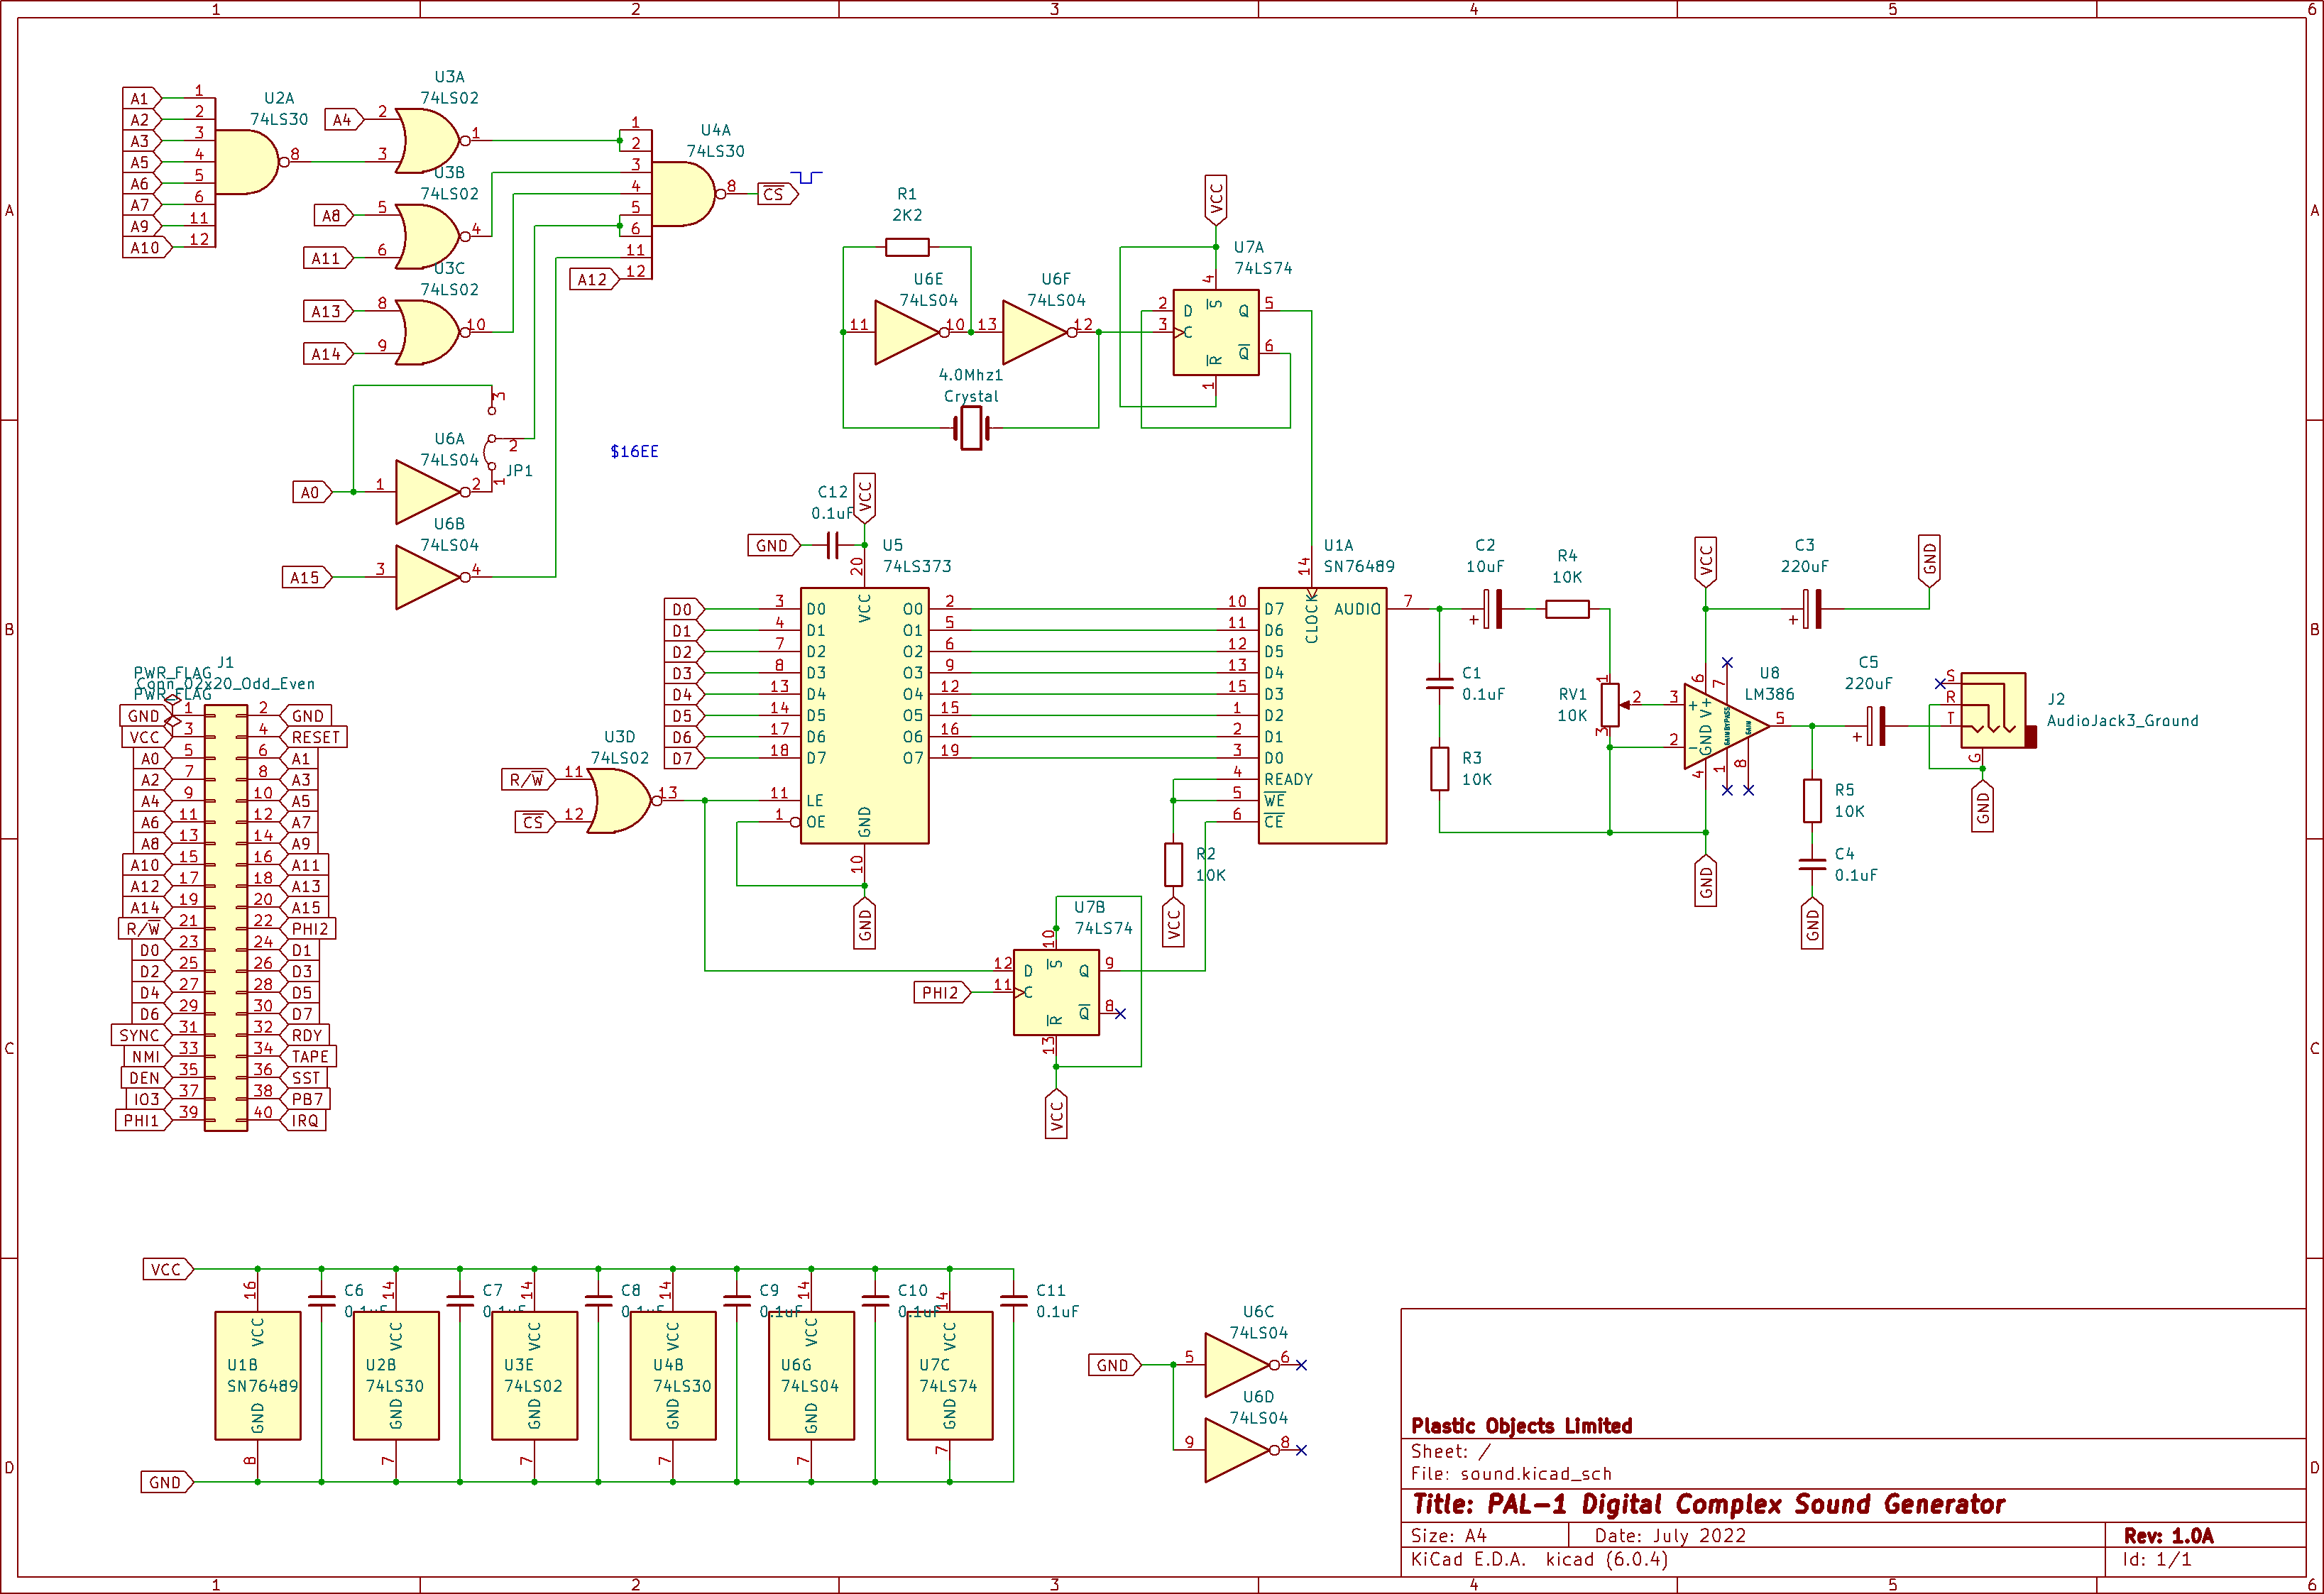
\includegraphics[width=1.8\textwidth,angle=90]{figures/schematic.png}
    }
\end{figure}
\end{document} 

\chapter{Board layout}
\begin{figure}[h!]
\centering
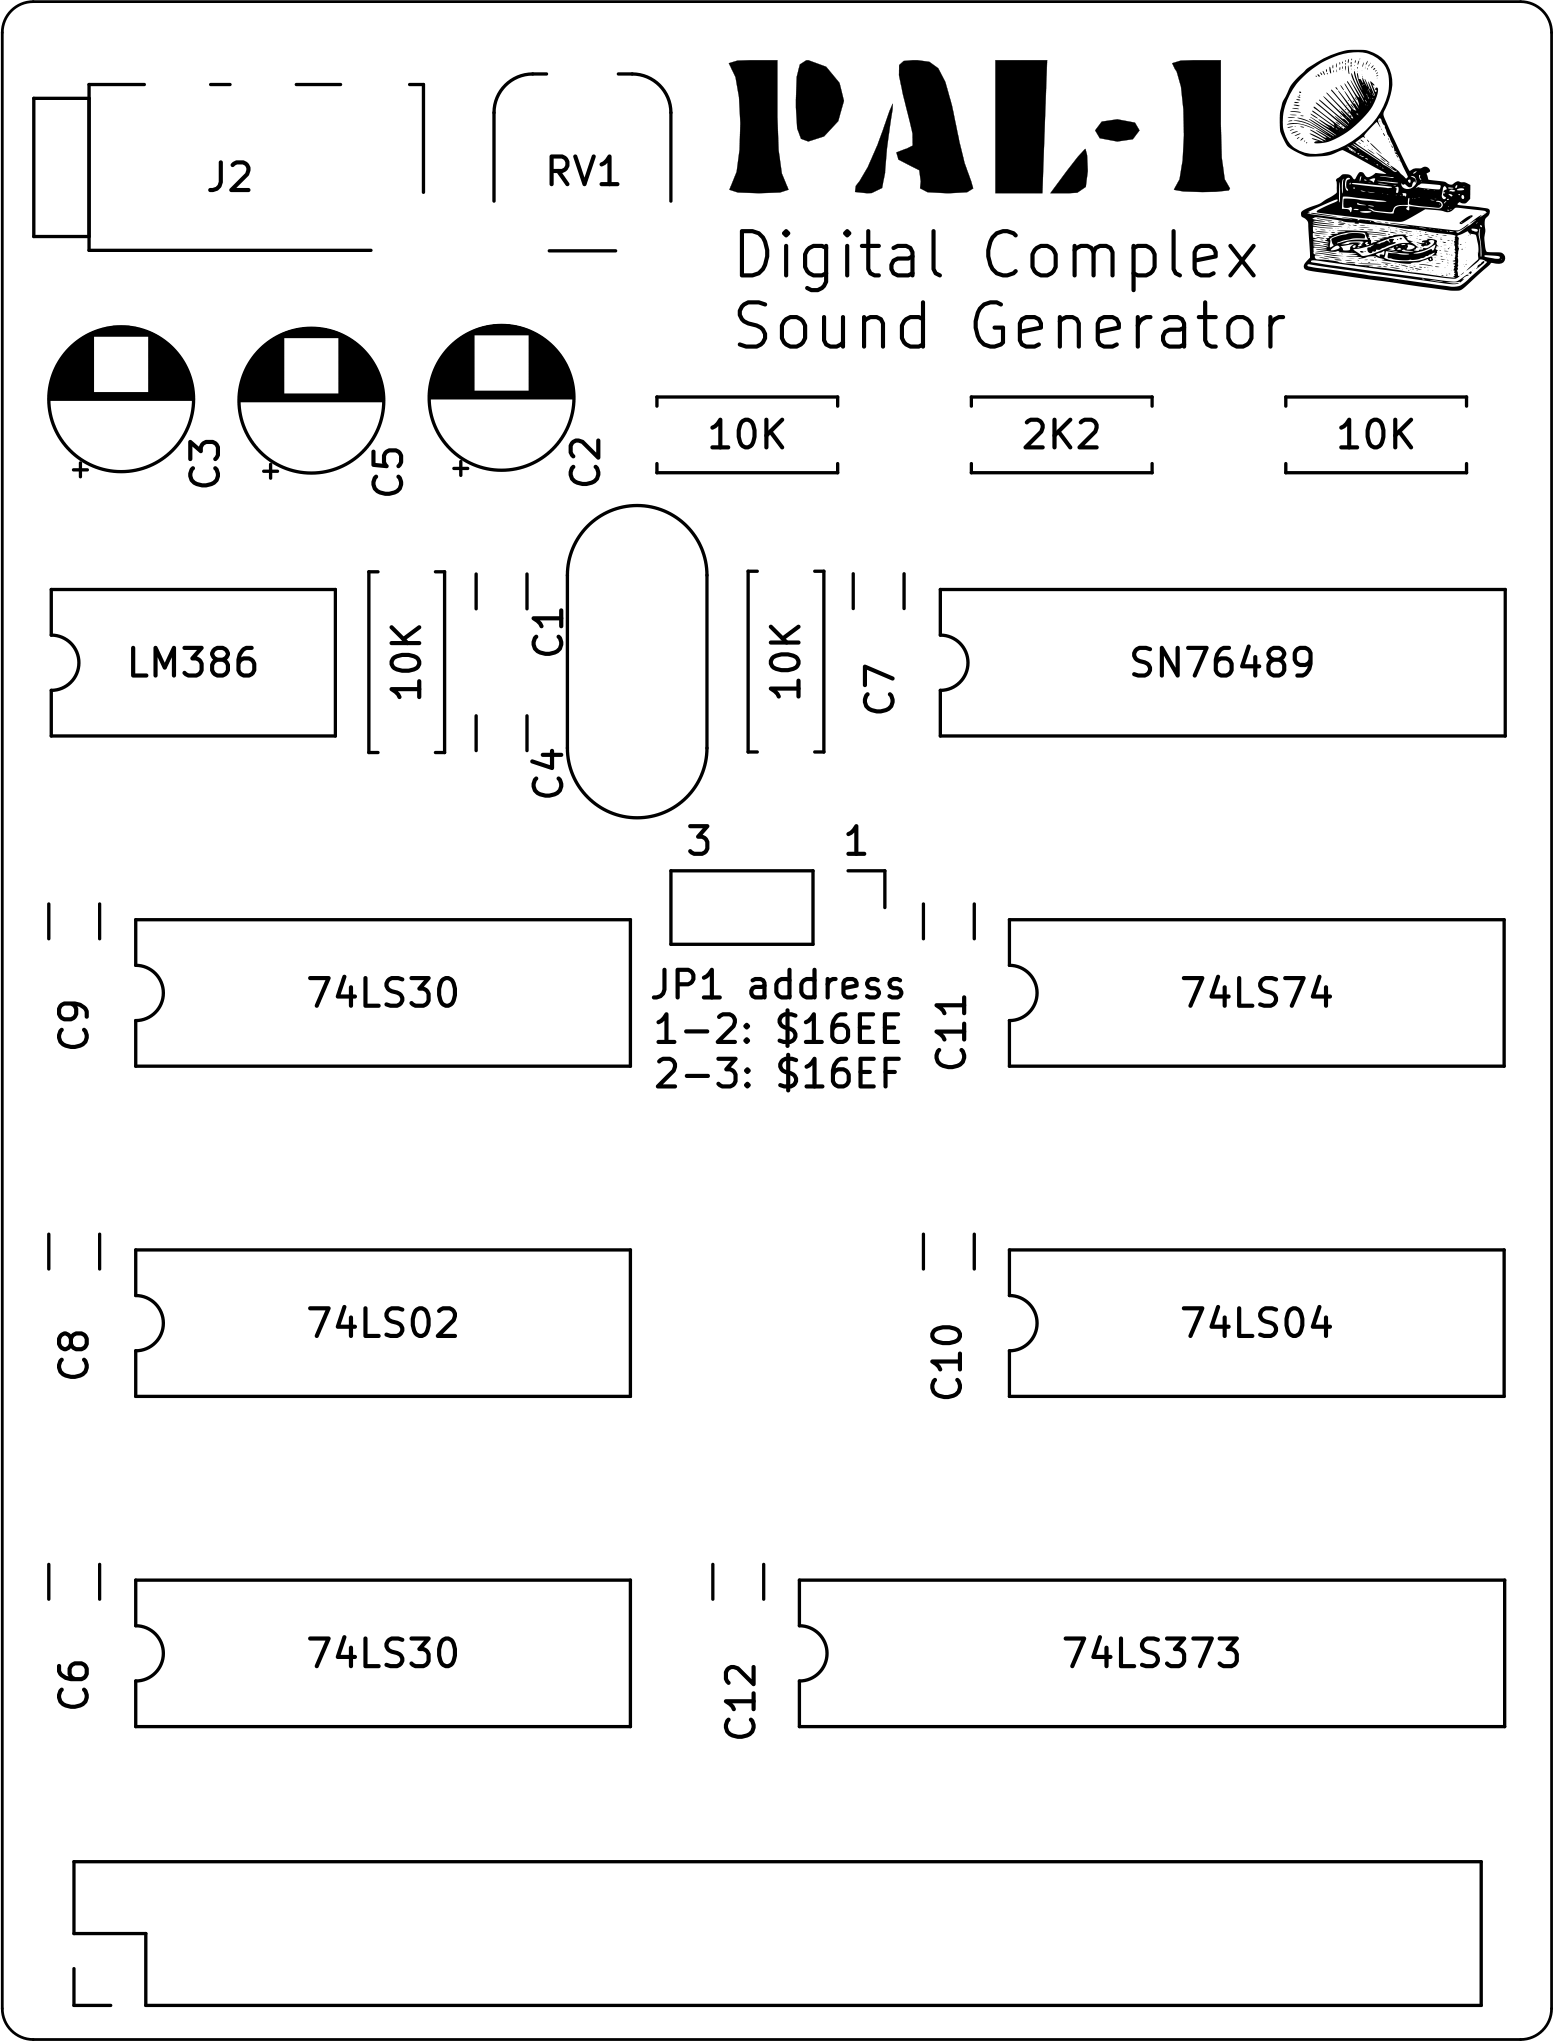
\includegraphics[scale=0.2]{figures/sound-brd-1.0a.png}
\end{figure}

\documentclass[a4paper,11pt]{article}
\usepackage[lmargin=142pt,rmargin=95pt,tmargin=127pt,bmargin=123pt]{geometry}
\usepackage[table]{xcolor}
\usepackage{csvsimple}
\usepackage{caption}
\newcommand{\chapter}{\section*}
\captionsetup[table]{labelformat=empty}
\begin{document}
\chapter{Bill of Materials}
\label{sec:bom}
\begin{table}[htb]
\csvreader[head to column names,
	tabular={| c | c | c | p{7cm} |},
	table head=\hline\rowcolor{gray!20}\textbf{Part} & \textbf{Qty} & \textbf{Value} & \textbf{Description}\\\hline,
	late after last line=\\\hline]{bom-v1_0A.csv}{}
	{\ref&\qty&\val&\component}  
\caption{PAL-1 Digital Complex Sound Generator V1.0A components}
\label{tab:bom}  
\end{table}
\end{document} 


\end{document}